\chapter{Performance metrics} \label{appx:perf}

This appendix presents performance metrics for the desktop application
implemented using the \emph{High performance C++ Profiler}. For further
details refer to section~\ref{sec:results:perf}.

Each performance metric contains two tables. The first is ordered by
function structure and total cycles the CPU spent on that function. The second
table is ordered by self cycles, which represents the total cycles the CPU spent
on that function minus the total cycles the CPU spent on the children functions.

The short descriptions of the performance metrics and the page number
where each can be found follows:

\newcommand{\profile}[1]{% index
  \ifnumequal{#1}{1}{
    Initial performance metrics.
  }{}
  \ifnumequal{#1}{2}{
    Performance metrics using faster resize operations.
  }{}
  \ifnumequal{#1}{3}{
    Performance metrics when face detection was executed every 10 frames
    instead of every frame.
  }{}
  \ifnumequal{#1}{4}{
    Performance metrics with no \emph{resize face box} and
    \emph{resize and draw face box back to frame} operations since the
    \emph{EvmGdownIIR} implementation always resizes to a predefined size.
  }{}
}

\begin{description}
  \item[Appendix \ref{pdf:profile:1} on page~\pageref{pdf:profile:1}]\hfill\\\profile{1}
  \item[Appendix \ref{pdf:profile:2} on page~\pageref{pdf:profile:2}]\hfill\\\profile{2}
  \item[Appendix \ref{pdf:profile:3} on page~\pageref{pdf:profile:3}]\hfill\\\profile{3}
  \item[Appendix \ref{pdf:profile:4} on page~\pageref{pdf:profile:4}]\hfill\\\profile{4}
\end{description}

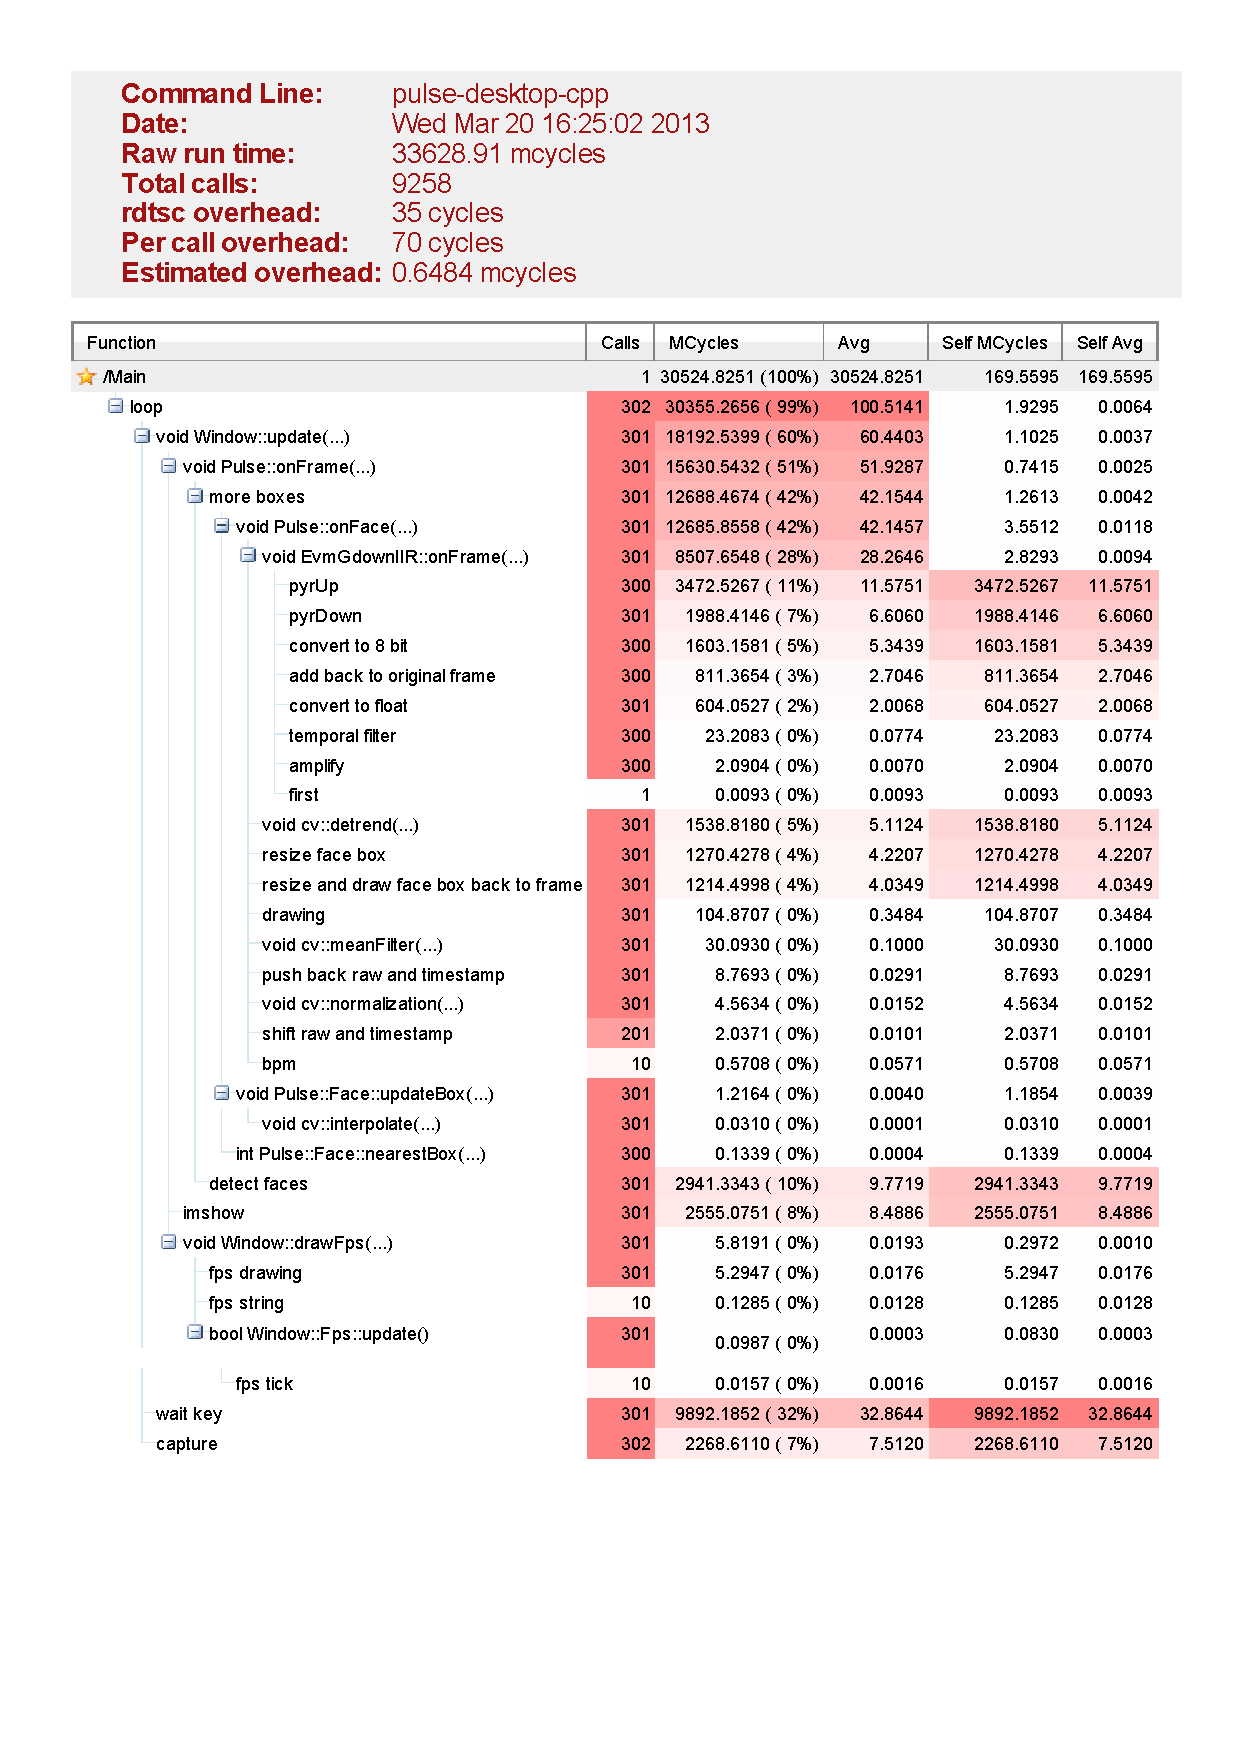
\includepdf[
  pages=-,
  pagecommand={\thispagestyle{plain}},
  addtolist={1, table, \profile{1}, pdf:profile:1}
]{profile/1}

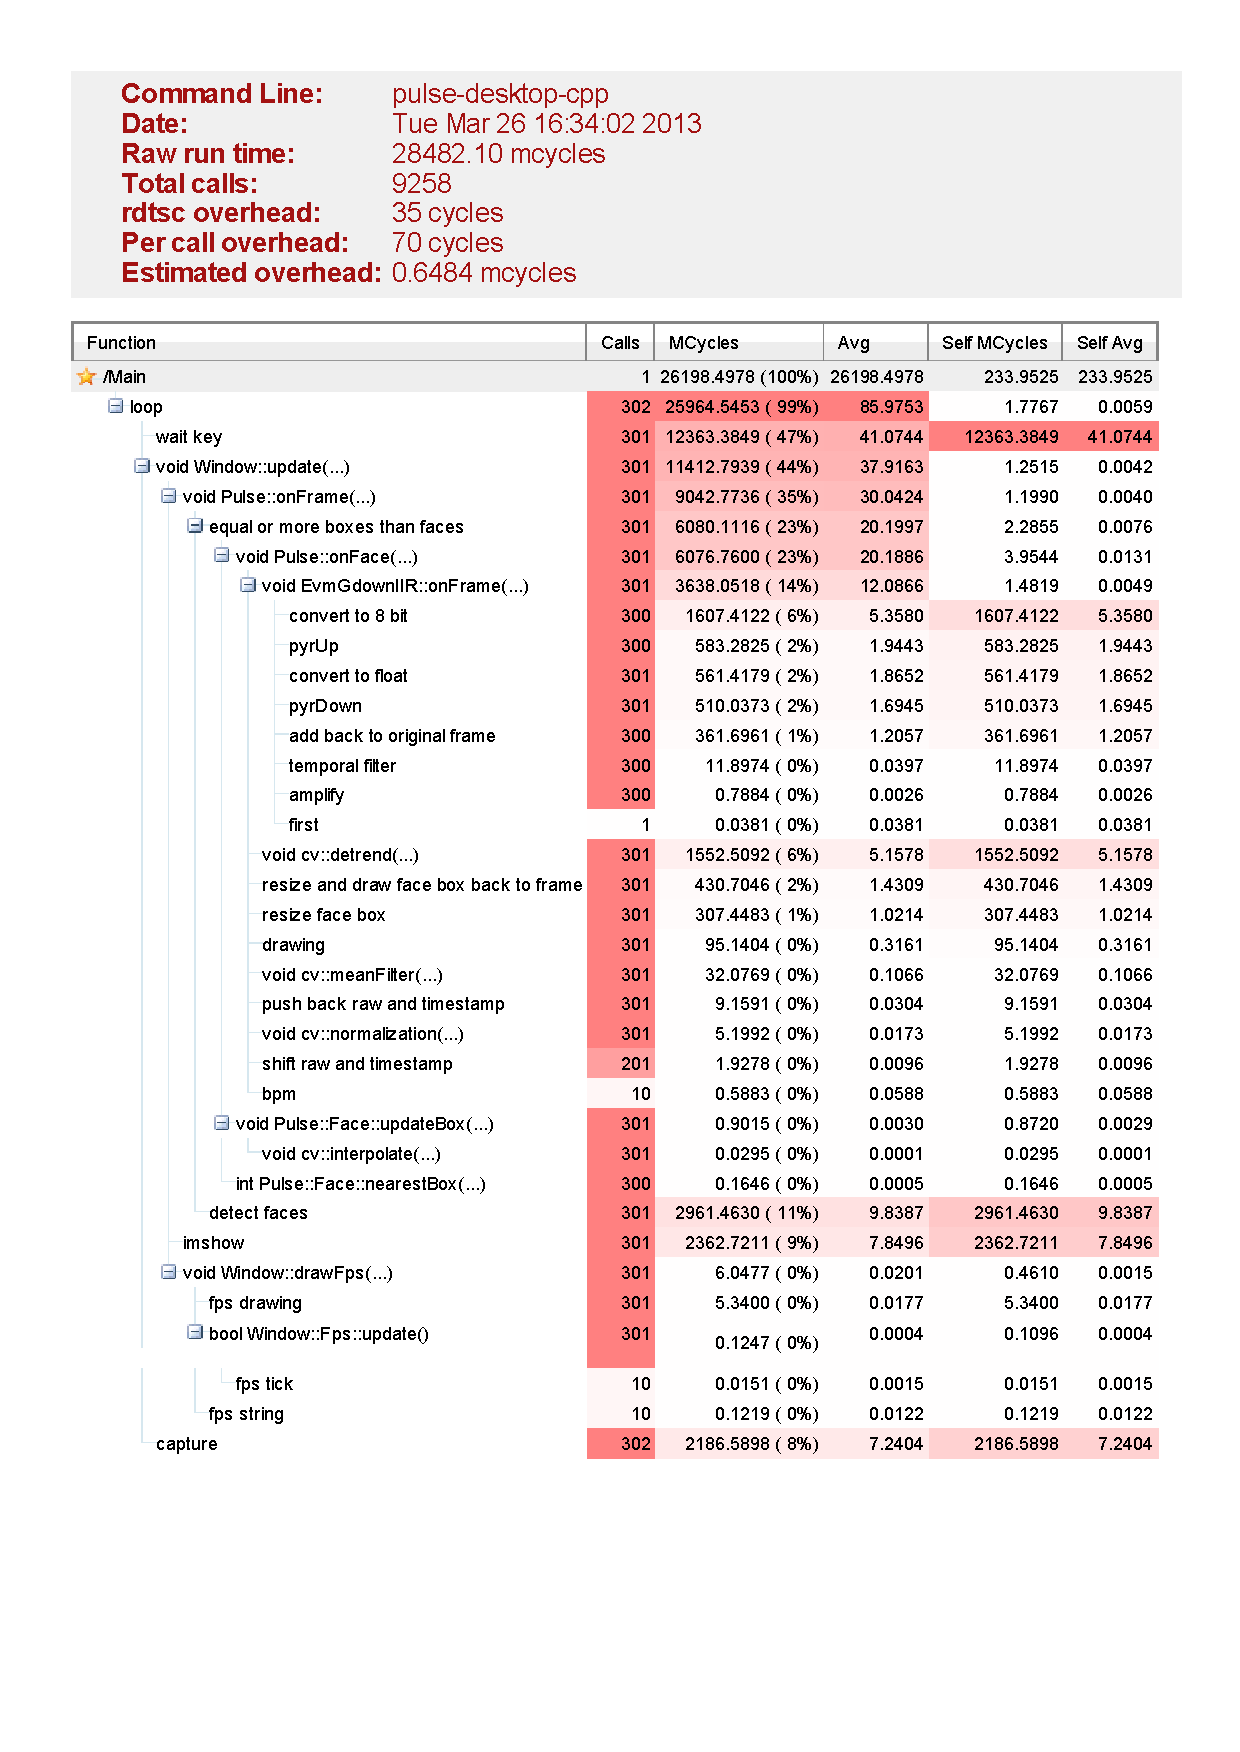
\includepdf[
  pages=-,
  pagecommand={\thispagestyle{plain}},
  addtolist={1, table, \profile{2}, pdf:profile:2}
]{profile/2}

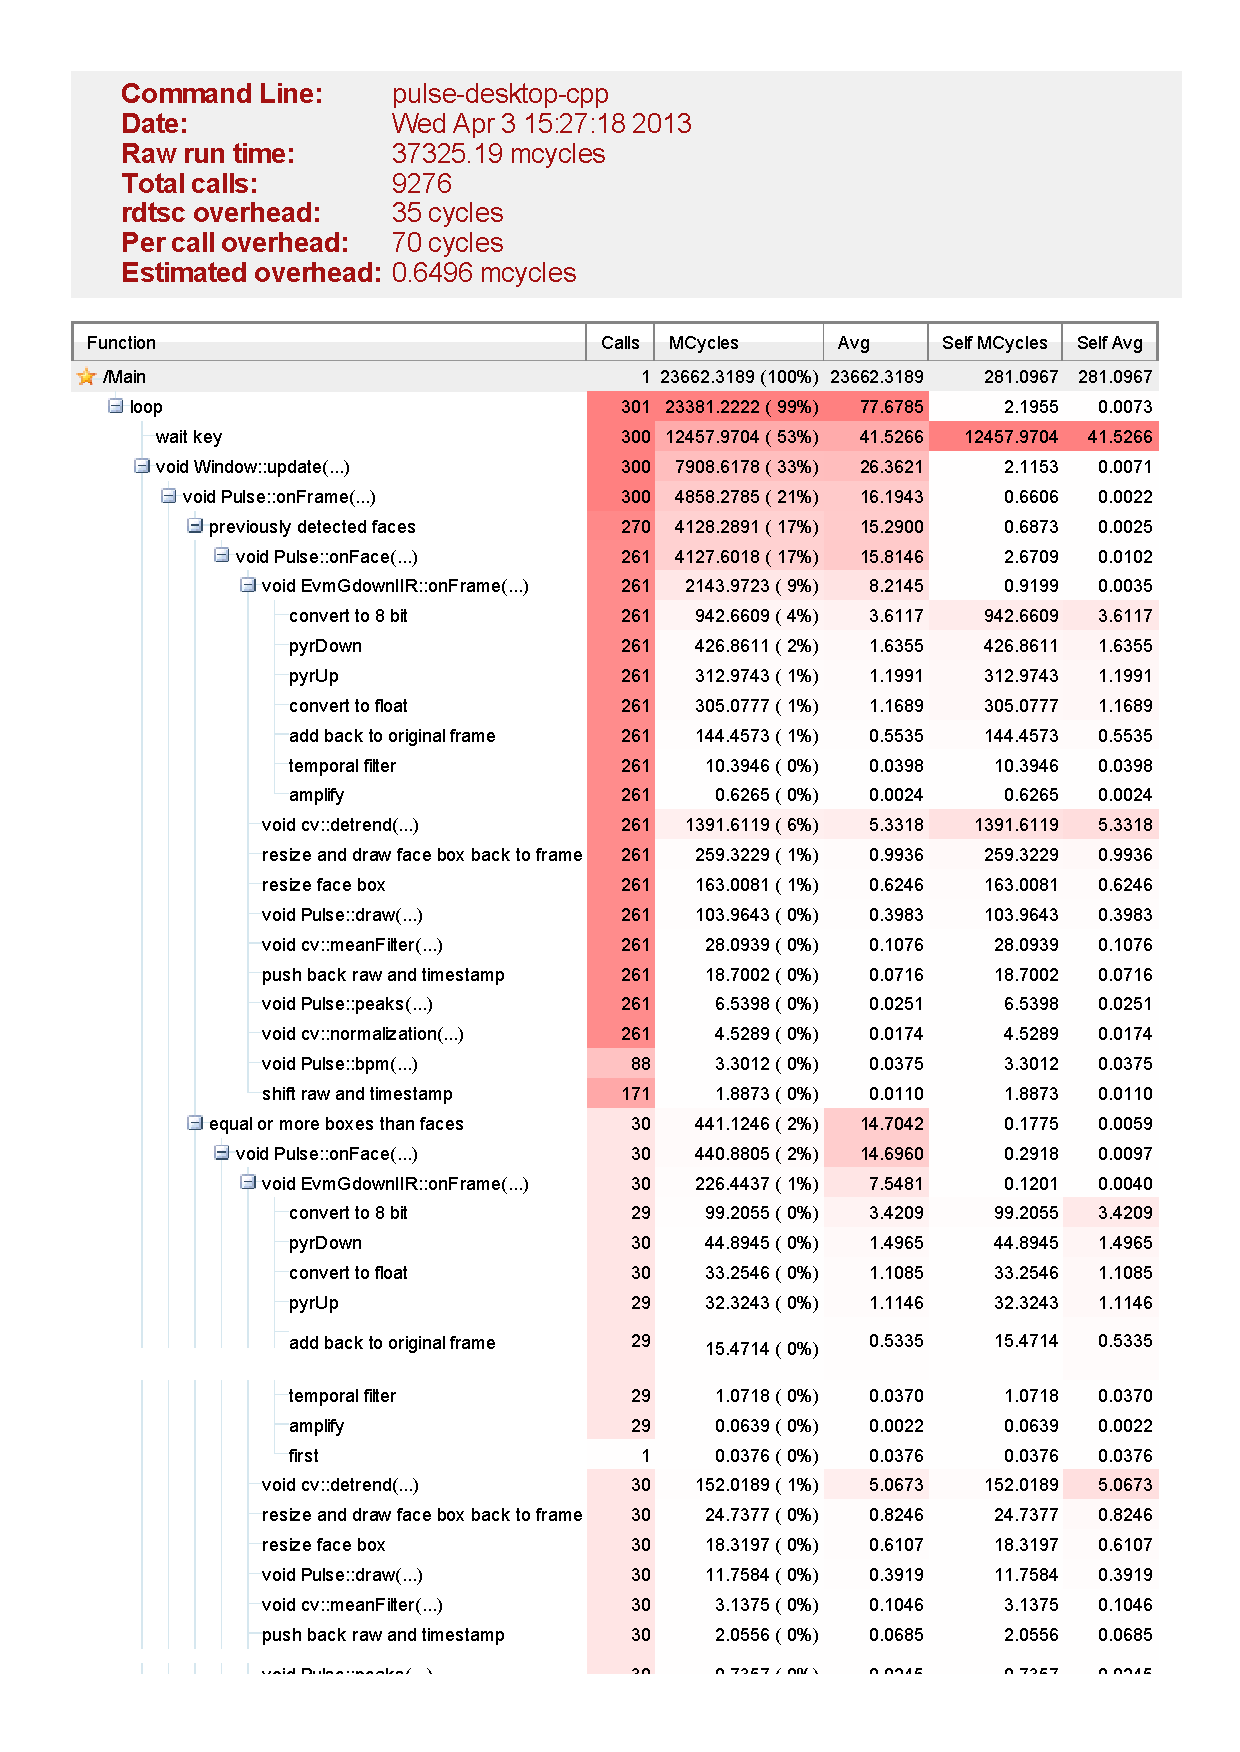
\includepdf[
  pages=-,
  pagecommand={\thispagestyle{plain}},
  addtolist={1, table, \profile{3}, pdf:profile:3}
]{profile/3}

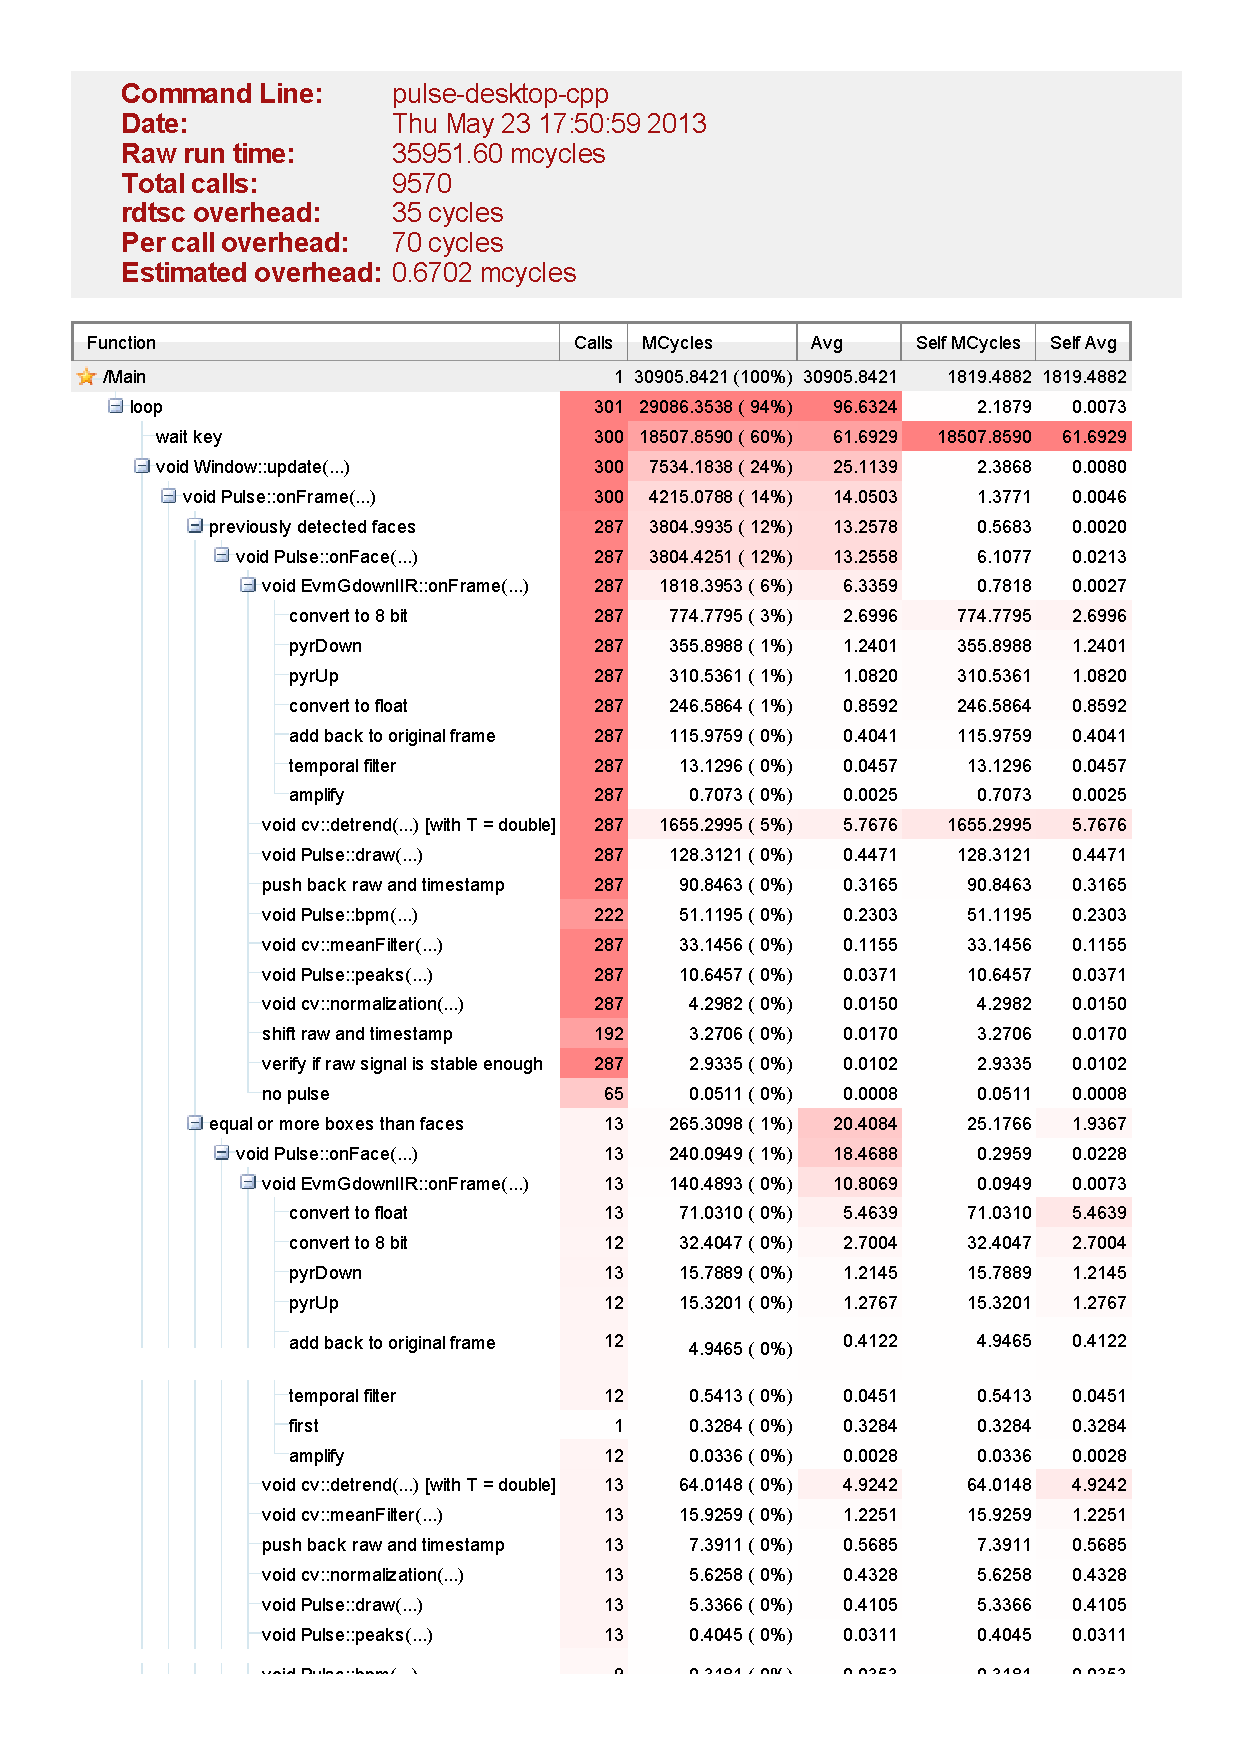
\includepdf[
  pages=-,
  pagecommand={\thispagestyle{plain}},
  addtolist={1, table, \profile{4}, pdf:profile:4}
]{profile/4}
